%-*- coding: utf-8 -*-
\label{chap:pratiques}

\paragraph{Notions :} visualisation de données, représentativité des données,
équité des algorithmes, confidentialité des données, anonymisation,
responsabilité.

\paragraph{Objectifs pédagogiques :} 
\begin{itemize}      
  \setlength{\itemsep}{3pt}
\item S'interroger sur la pertinence d'une analyse de données et la validité
  des conclusions qui en sont tirées.
\end{itemize}

La science des données n'est pas uniquement une discipline technique : comme
souvent en ingénierie, nous ne pouvons pas dissocier les calculs que nous
faisons de la question posée ni de leur utilisation. Ce chapitre n'a pas
vocation à être un cours d'éthique% \footnote{L'éthique peut être définie comme
  % l'étude de la justification d'ue action à partir de normes, règles juridiques
  % ou déontologiques, valeurs morales, intuitions et traditions qui peuvent être
  % multiples et contradictoires au sein d'une même société.}
, mais à vous donner
quelques points d'entrée pour vous amener à vous poser des questions sur
l'usage de la science des données, de l'apprentissage automatique et de
l'intelligence artificielle. Pour cette raison, vous trouverez plus de liens
externes (cliquables dans la version PDF de ce document) qu'à l'habitude à
travers le texte de ce chapitre, pointant tant vers des publications
scientifiques que des blogs de vulgarisation ou des articles de presse grand
public. N'hésitez pas à poursuivre vos propres lectures sur le sujet.

Nous motiverons ce chapitre par deux citations : la première, attribuée à
Benjamin Disraeli par Mark Twain, ``\textit{There are three kinds of lies:
  lies, damned lies, and statistics}'', et la seconde, attribuée à George
Box, ``\textit{All models are wrong, but some are useful}''.

\section{Visualisation de données}
La façon dont vous choisissez de représenter vos données ou vos résultats a un
impact fort sur le message que vous essayez de faire passer. 

Mi-mai 2020, le Department of Public Health de l'État de Géorgie (États-Unis
d'Amérique) a publié le diagramme en barres de la
figure~\ref{fig:georgia_wtf_barplot}. Regardez bien l'axe des abscisses : le
message vous semble-t-il le même quand les dates sont ordonnées de manière
chronologique, comme sur la figure~\ref{fig:georgia_fixed_barplot} ?

\begin{figure}[h]
  \centering
  \begin{subfigure}[t]{0.47\textwidth}
    \centering
    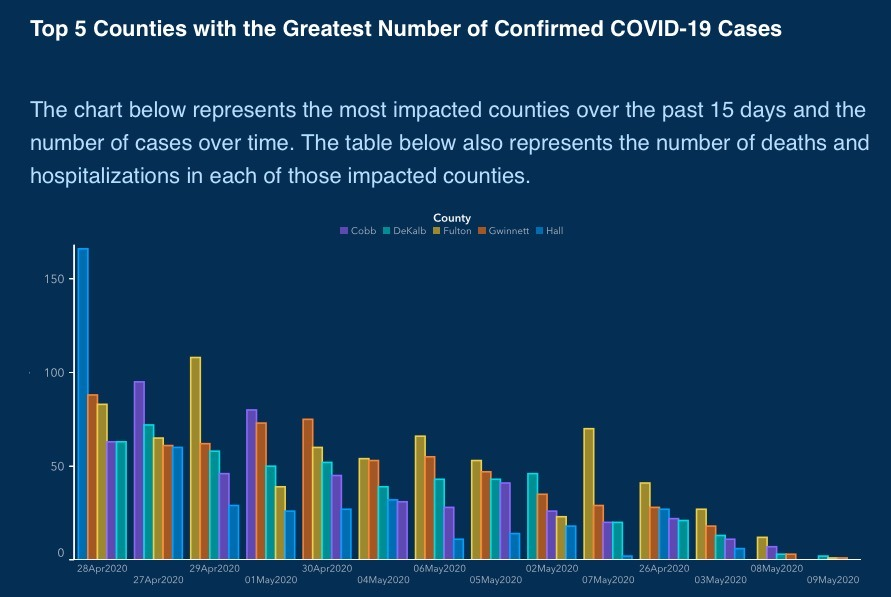
\includegraphics[width=\textwidth]{figures/pratiques/georgia_wtf_barplot}
    \caption{Première version du diagramme en barres.}
    \label{fig:georgia_wtf_barplot}
  \end{subfigure} \hfill
  \begin{subfigure}[t]{0.47\textwidth}
    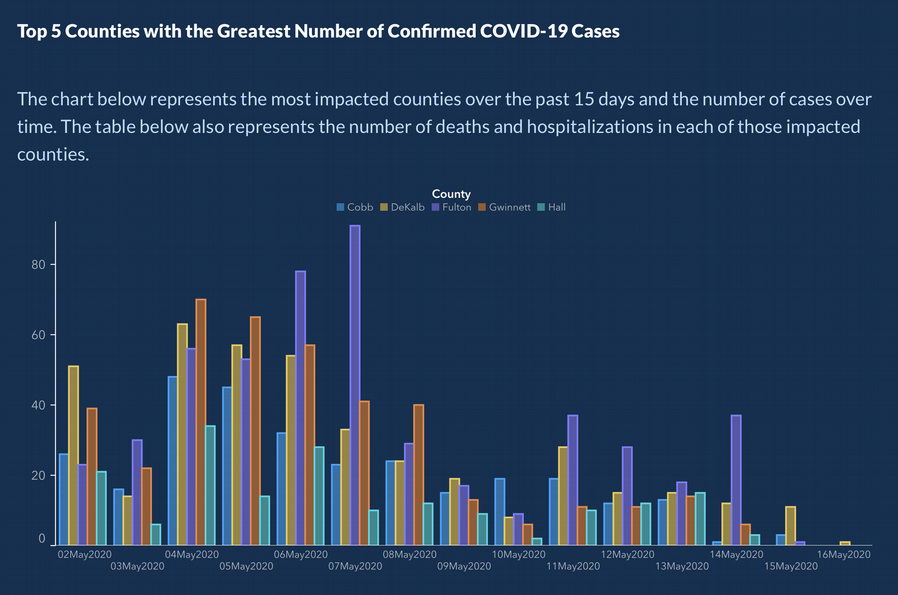
\includegraphics[width=\textwidth]{figures/pratiques/georgia_fixed_barplot}  
    \caption{Deuxième version du diagramme en barres.}
    \label{fig:georgia_fixed_barplot}
  \end{subfigure}  
  \caption{Deux variantes du même diagramme en barres publiées par le
    Department of Public Health de l'État de Géorgie à propos du nombre de cas
    de CoVid19.}
  %\label{fig:georgia_barplot}
\end{figure}

Il est donc très important de vous assurez que vos graphiques soient lisibles
et qu'ils traduisent clairement votre message sans déformer les données. La
visualisation des données, ou \textit{dataviz}, est un champ d'études à part
entière.  Nous nous contenterons ici de citer quelques principes parmi les plus
importants.

\subsection{Des graphiques clairs et lisibles}
Un bon graphique doit pouvoir être compréhensible de manière autonome,
c'est-à-dire sans référence au texte. Pour cela, quelques éléments généraux,
valables bien au-delà de ce cours :
\begin{itemize}
\item Pour être compréhensible, un graphique doit comporter un certain nombre
  d'éléments indispensables à sa compréhension, et en particuilier :
  \begin{itemize}
  \item un titre ;
  \item une légende ;
  \item le nom des axes, l'unité des variables représentées, et l'échelle si
    elle n'est pas linéaire (par exemple, échelle logarithmique).
  \end{itemize}
\item Pour qu'un graphique soit lisible, ses éléments doivent être suffisamment
  grands. Attention en particulier à :
  \begin{itemize}
  \item la taille des textes (légendes, graduations, etc.) ;
  \item la taille des marqueurs et l'épaisseur des traits.
  \end{itemize}
\item Pour être lisible, un graphique ne doit pas comporter d'éléments
  superflus. En particulier, il vaut mieux éviter
  \begin{itemize}
  \item de représenter trop d'informations/éléments à la fois ;
    il est difficile de garder en mémoire plus de 7--10 éléments à la fois ;
  \item d'utiliser trop de couleurs différentes, surtout si elles ne
    contiennent pas d'information.
  \end{itemize}
\end{itemize}

\subsection{Choix des axes}
%https://callingbullshit.org/tools/tools_misleading_axes.html 
Le choix des échelles et intervalles d'un graphique a une influence sur son
interprétation.

Pour un diagramme en barres, ne pas faire commencer les axes à 0 peut
artificiellement gonfler les différences entre les différentes barres. Ainsi,
le diagramme de la figure~\ref{fig:bars_start_nonzero} indique que le modèle 4
est bien supérieur aux autres, tandis que celui de la
figure~\ref{fig:bars_start_zero} montre des performances très comparables entre
les différentes méthodes. (Dans ce cas précis, il serait de toute façon
souhaitable de répéter plusieurs fois l'entrainement et l'évaluation, par
exemple avec une validation croisée (que nous verrons
section~\ref{sec:crossval}) et de produire des barres d'erreurs.)
\begin{figure}[h]
  \centering
  \begin{subfigure}[t]{0.47\textwidth}
    \centering
    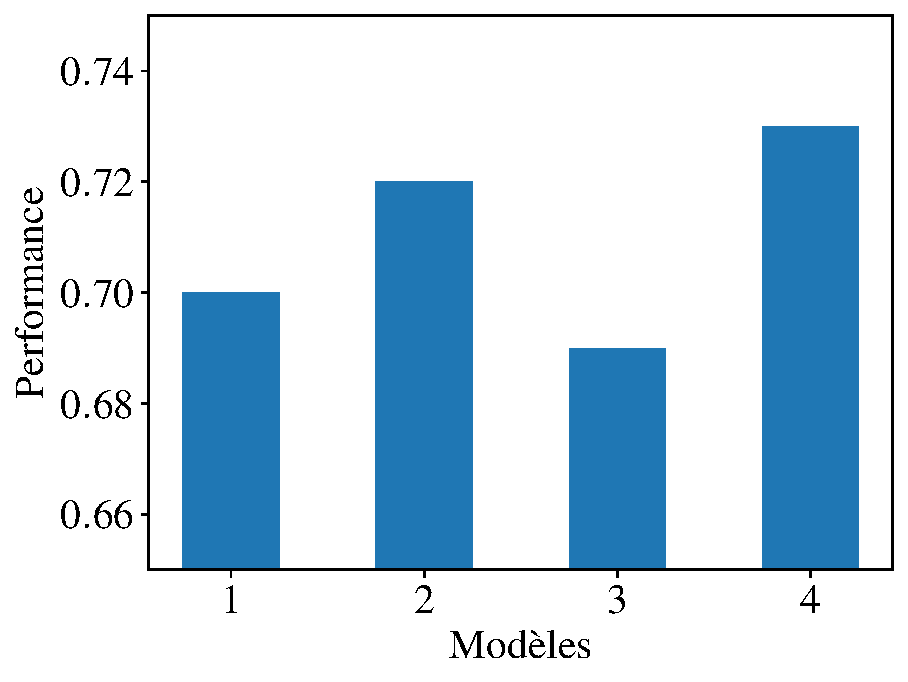
\includegraphics[width=\textwidth]{figures/pratiques/bars_start_nonzero}
    \caption{Axe des ordonnées réduit.}
    \label{fig:bars_start_nonzero}
  \end{subfigure} \hfill
  \begin{subfigure}[t]{0.47\textwidth}
    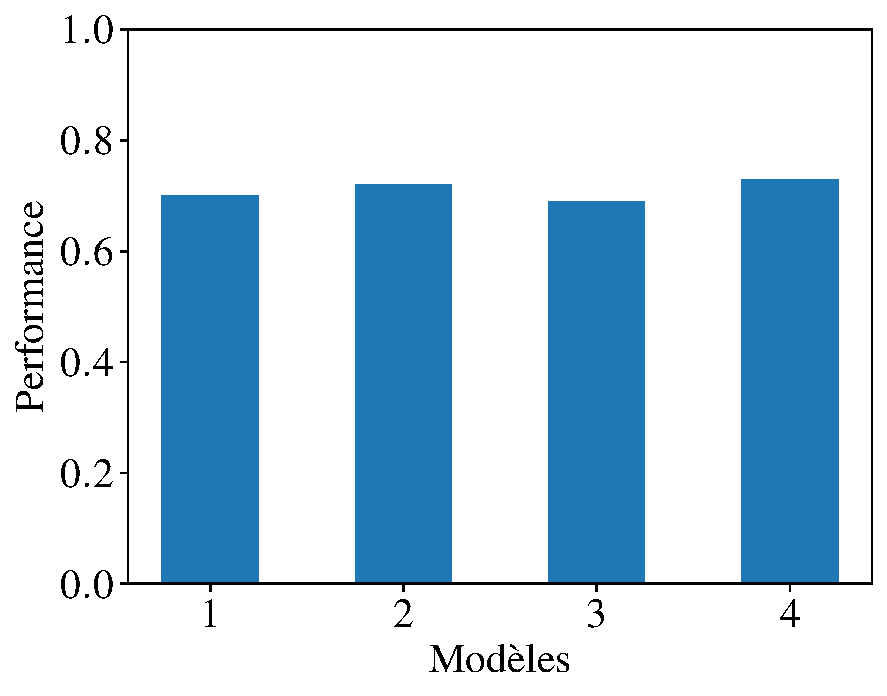
\includegraphics[width=\textwidth]{figures/pratiques/bars_start_zero}  
    \caption{Axe des ordonnées allant de 0 à 1.}
    \label{fig:bars_start_zero}
  \end{subfigure}  
  \caption{Deux façons de présenter la comparaison des performances de 4 modèles.}
  %\label{fig:georgia_barplot}
\end{figure}

À l'inverse, il pourra être préférable pour un diagramme dont le but est non
pas de comparer les valeurs absolues de variables mais plutôt de présenter leur
évolution que l'axe des ordonnées ne commence pas à zéro. Ainsi, la
figure~\ref{fig:line_start_zero} indique une température très stable, tandis
que la figure~\ref{fig:line_start_nonzero} permet de mieux rendre compte des
variations.
\begin{figure}[h]
  \centering
  \begin{subfigure}[t]{0.47\textwidth}
    \centering
    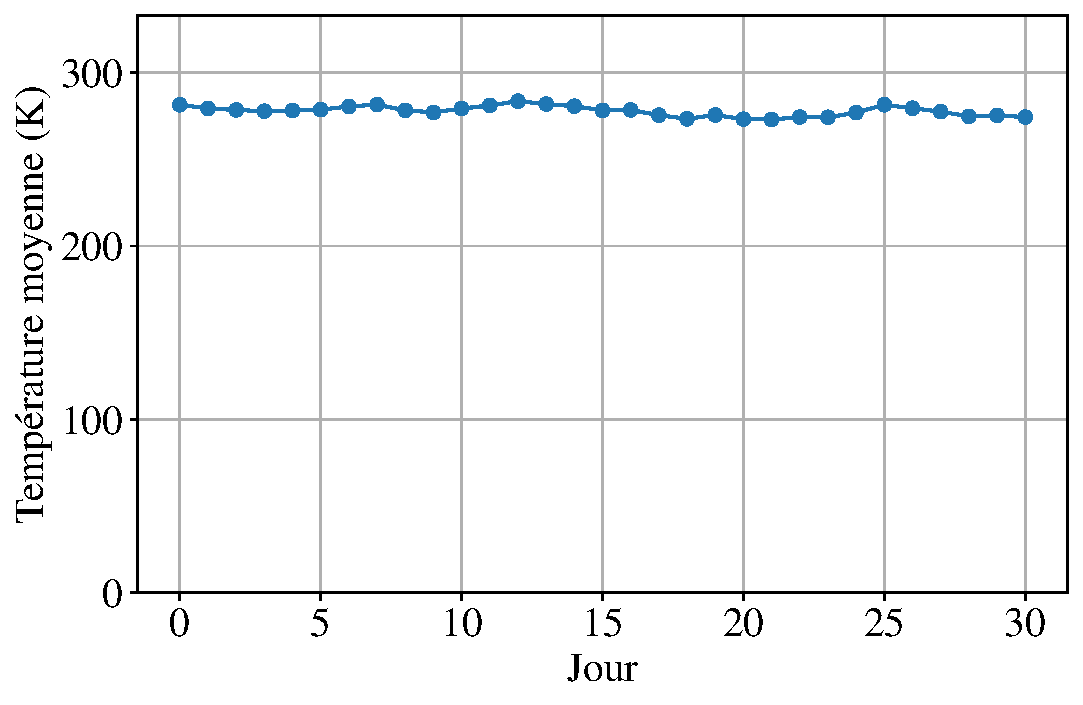
\includegraphics[width=\textwidth]{figures/pratiques/line_start_zero}
    \caption{Axe des ordonnées partant de 0K.}
    \label{fig:line_start_zero}
  \end{subfigure} \hfill
  \begin{subfigure}[t]{0.47\textwidth}
    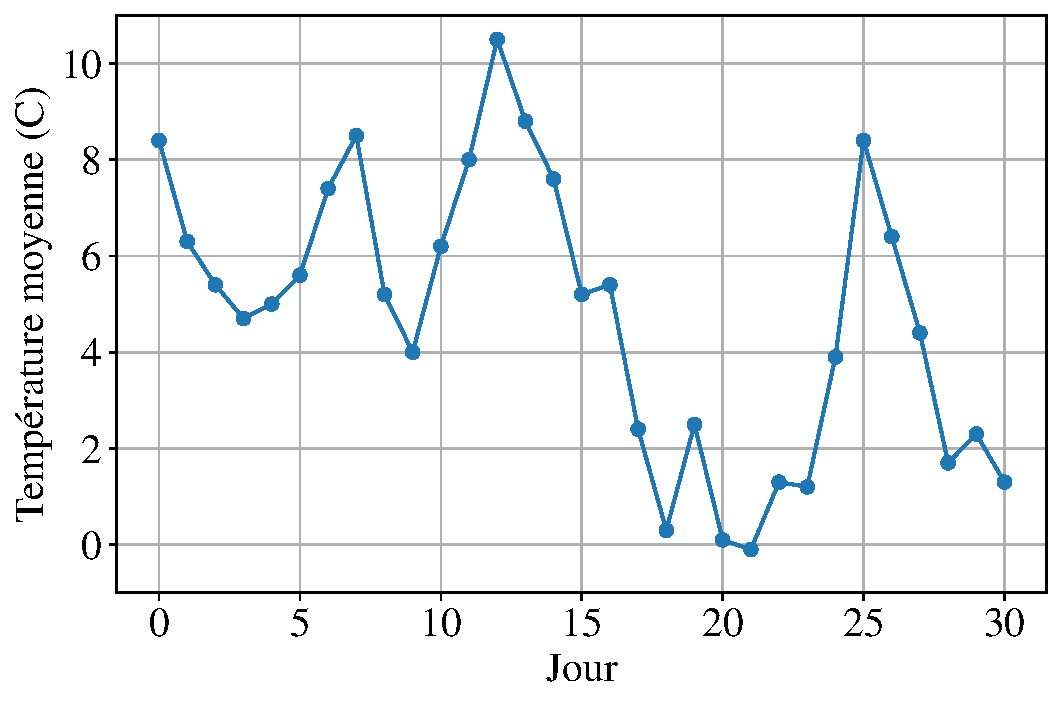
\includegraphics[width=\textwidth]{figures/pratiques/line_start_nonzero}  
    \caption{Axe des ordonnées réduit.}
    \label{fig:line_start_nonzero}
  \end{subfigure}  
  \caption{Deux façons de présenter l'évolution des températures moyenne de la
    table~\ref{tab:meteo_data}.}
  %\label{fig:georgia_barplot}
\end{figure}

\subsection{\textit{Proportional ink} ou principe de l'encre proportionnelle}
%https://callingbullshit.org/tools/tools_proportional_ink.html
De manière générale, il est recommandé, lorsque l'on utilise des surfaces pour
représenter des nombres (par exemple, les rectangles d'un diagramme en barres),
que ces surfaces soient d'aires pro\-por\-tion\-nel\-les aux nombres en question. On
retrouve d'ailleurs ici l'idée de commencer les barres d'un diagramme en
barres à 0.

Il faut cependant faire aussi attention à ce que les surfaces en question
soient faciles à comparer visuellement. Un diagramme camembert est ainsi
préférable à un graphique à bulles ; mais un diagramme en barres est
généralement plus lisible qu'un diagramme camembert. La figure~\ref{fig:areas}
l'illustre. Il s'agit d'une variante d'une
expérience
  menée au début des années 1980 (\href{https://www.jstor.org/stable/2288400}{William S. Cleveland \& Robert McGill, 1984}) et souvent considérée comme fondatrice en
\textit{dataviz}.

Remarquez ici que le diagramme en barres serait encore plus lisible sans couleurs (elles n'apportent rien) et en ordonnant les catégories par proportion.
\begin{figure}[h]
  \centering
  \begin{subfigure}[t]{0.20\textwidth}
    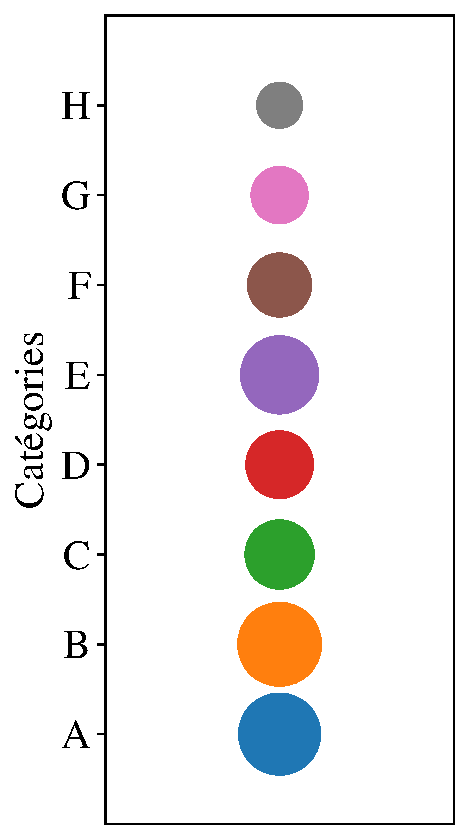
\includegraphics[width=\textwidth]{figures/pratiques/areas_bubbles}  
    \caption{Graphique à bulles.}
    \label{fig:areas_bubbles}
  \end{subfigure}  \hfill
  \begin{subfigure}[t]{0.33\textwidth}
    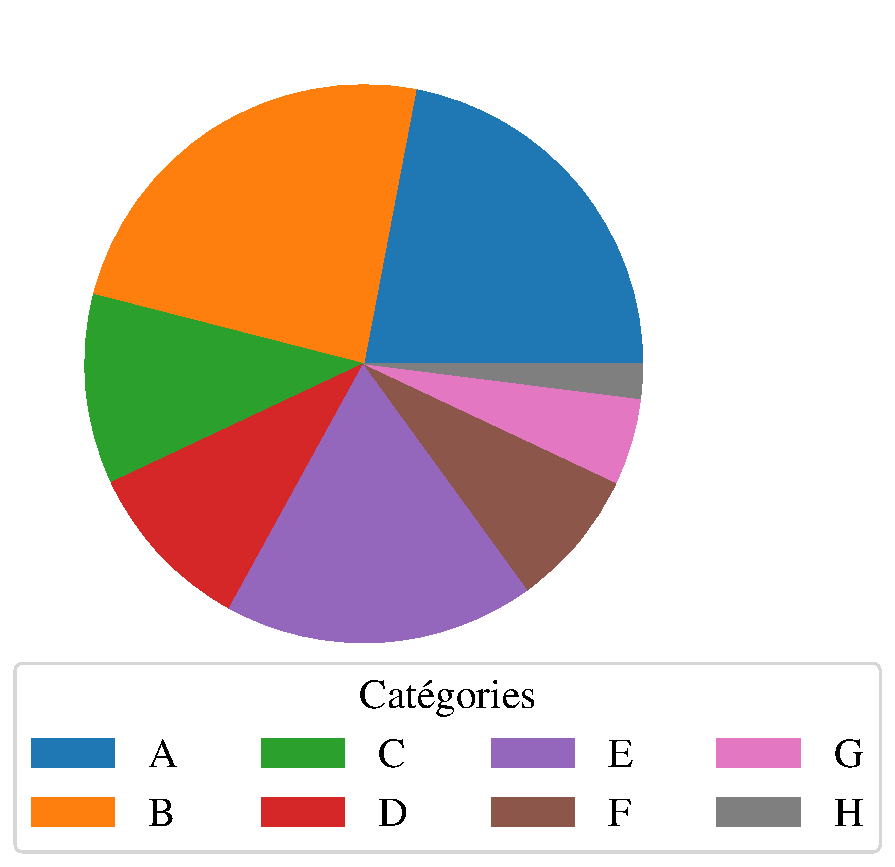
\includegraphics[width=\textwidth]{figures/pratiques/areas_pie}  
    \caption{Diagramme camembert.}
    \label{fig:areas_pie}
  \end{subfigure} \hfill
  \begin{subfigure}[t]{0.33\textwidth}
    \centering
    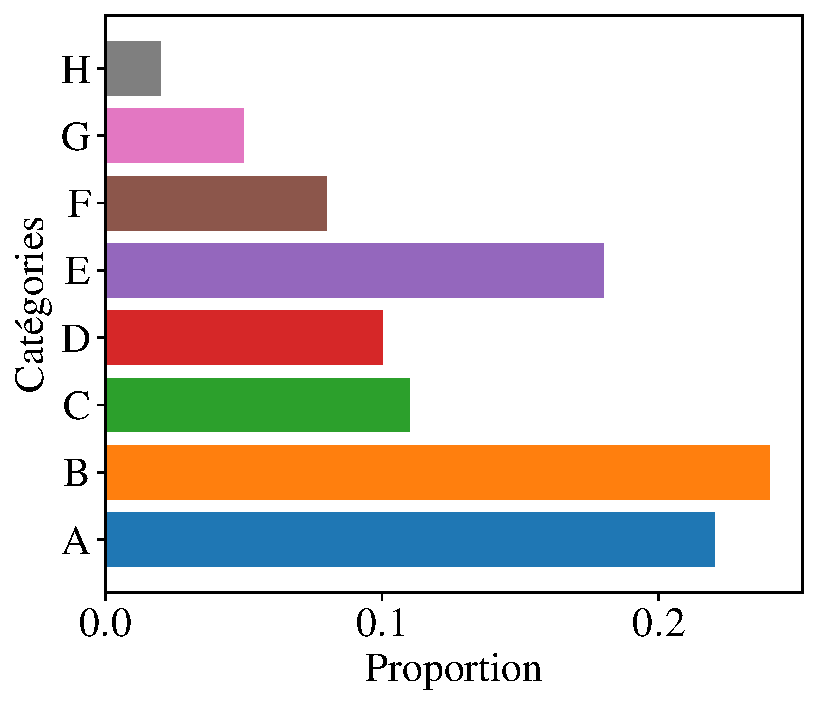
\includegraphics[width=\textwidth]{figures/pratiques/areas_bars}
    \caption{Diagramme en barres.}
    \label{fig:areas_bars}
  \end{subfigure} 
  \caption{Trois façons de représenter les proportions de 8 catégories. Quelle(s) représentation(s) permettent de les classer aisément par ordre croissant ?}
  \label{fig:areas}
\end{figure}

%\subsection{Attention aux résumés}
%https://python-graph-gallery.com/39-hidden-data-under-boxplot/ 


\subsection{Dyschromatopie}
Nous ne percevons pas les couleurs de la même façon. Une forte proportion de la population est atteinte d'une forme ou d'une autre de dyschromatopie, la plus fréquente étant la deutéranopie (incapacité à différencier rouge et vert). 

Pour assurer une accessibilité maximale, utilisez des échelles de couleurs
adaptées. Il est difficile de s'adapter à \textit{toutes} les dyschromatopies ;
néanmoins le cycle par défaut de \texttt{matplotlib} est supposé être
relativement adapté. Pour des \textit{heatmaps}, favoriser les échelles de
couleur \textit{viridis} ou \textit{cividis} (voir
figure~\ref{fig:pca_plot}). Des outils comme \href{https://www.color-blindness.com/coblis-color-blindness-simulator/}{CBLIS} ou \href{https://www.funkify.org}{Funkify} vous permettent de simuler différentes dyschromatopies pour vérifier la lisibilité de vos graphiques.

Vous pouvez aussi augmenter la lisibilité de vos graphiques en utilisant des
indices supplémentaires (épaisseur de trait, hachures, forme des points,
ordonner les légendes dans le même ordre que les courbes, etc.) et en doublant
vos images d'une description textuelle alternative pour les personnes
non-voyantes.


\begin{figure}[h]
  \centering
  \begin{subfigure}[t]{0.30\textwidth}
    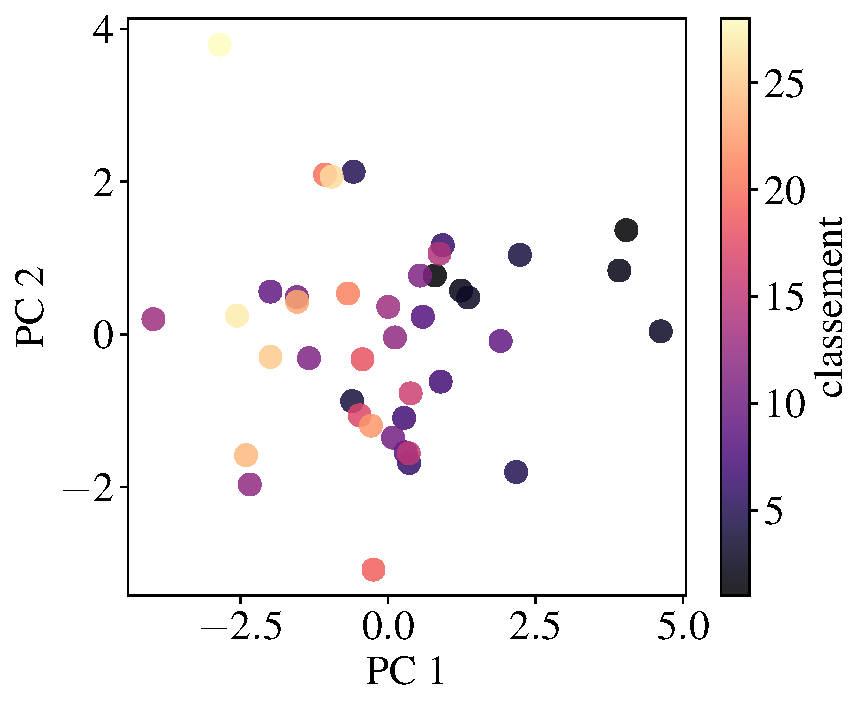
\includegraphics[width=\textwidth]{figures/pratiques/pca_plot_magma}  
    \caption{Magma.}
    \label{fig:pca_plot_magma}
  \end{subfigure}  \hfill
  \begin{subfigure}[t]{0.30\textwidth}
    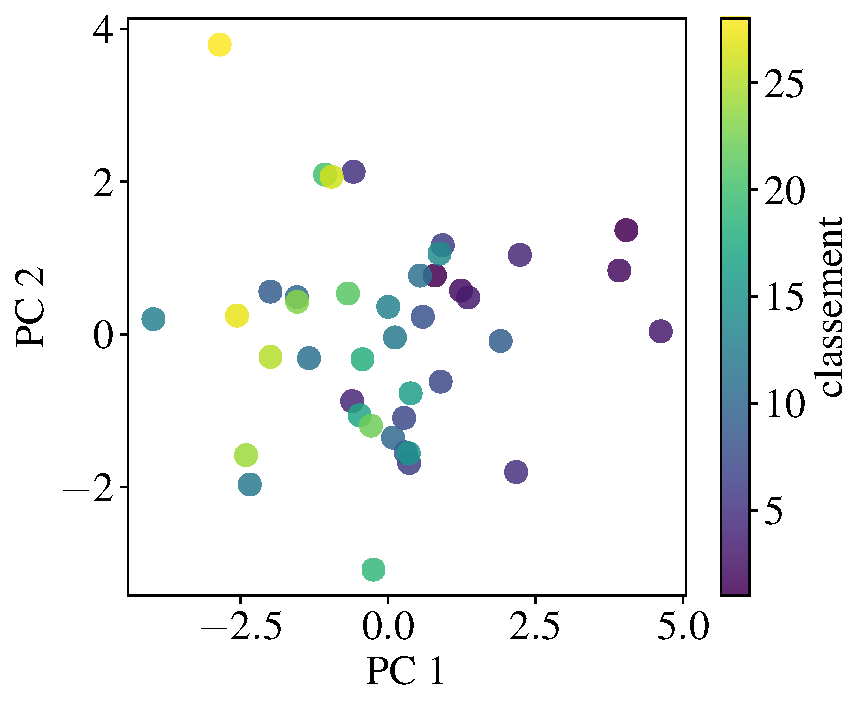
\includegraphics[width=\textwidth]{figures/pratiques/pca_plot_viridis}  
    \caption{Viridis.}
    \label{fig:pca_plot_viridis}
  \end{subfigure} \hfill
  \begin{subfigure}[t]{0.30\textwidth}
    \centering
    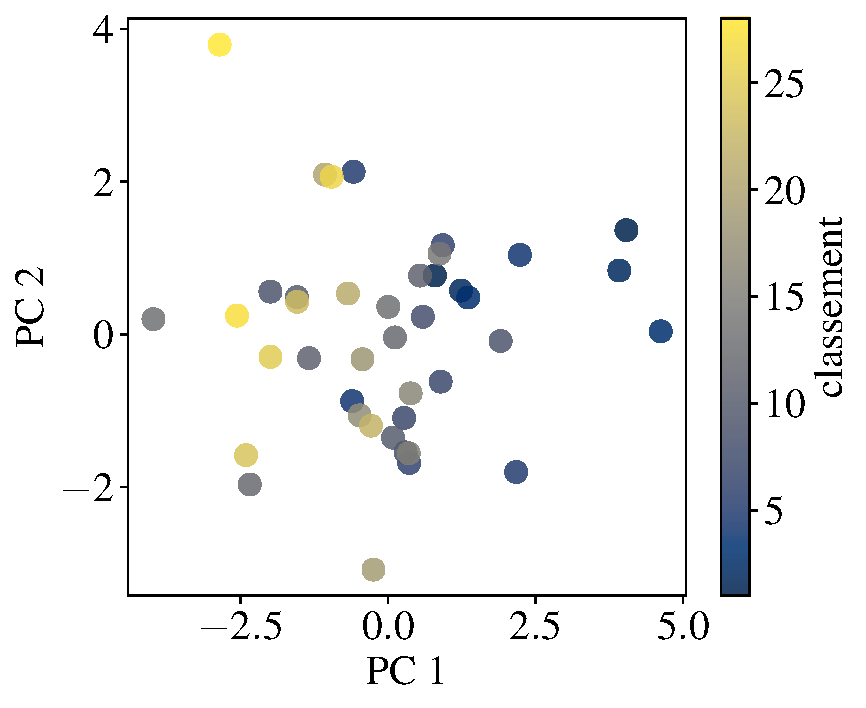
\includegraphics[width=\textwidth]{figures/pratiques/pca_plot_cividis}
    \caption{Cividis.}
    \label{fig:pca_plot_cividis}
  \end{subfigure} 
  \caption{Athlètes de la PC2, représentés selon deux composantes, et colorés
    en fonction de leur classement, selon trois échelles de couleur
    différentes.}
  \label{fig:pca_plot}
\end{figure}

\section{Équité des algorithmes}
Une question importante qui se pose constamment en science des données est
celle de la \textbf{reproduction des biais}. En effet, un modèle appris sur un
jeu de données peut facilement reproduire des biais de ce jeu de données,
qu'ils soient explicites ou implicites.

Un exemple qui revient souvent est celui d'un \href{https://www.numerama.com/tech/426774-amazon-a-du-desactiver-une-ia-qui-discriminait-les-candidatures-de-femmes-a-lembauche.html}{algorithme de ressources humaines
utilisé par Amazon en 2014.} Le modèle avait tendance à rejeter les candidatures posées
par des femmes. En effet, il était entraîné sur des données internes à
l'entreprise, dont les recrutements étaient fortement biaisés en faveur des
hommes. Bien que le genre n'ait pas été une variable utilisée pour décrire les
candidatures, le modèle détectait dans le texte des CV des informations
corrélée dans le jeu d'entraînement au rejet d'une candidature mais qui
s'avéraient surtout traduire qu'elle était posée par une femme (éducation dans
un établissement non-mixte réservé aux femmes ; appartenance à une équipe de
sport féminin, etc.). Ces biais sont toujours présents dans les modèles de
language actuels, comme le montre une étude récente (\href{https://arxiv.org/abs/2504.21400}{Sugat Chaturvedi \& Rochana Chaturvedi, 2025}).

Ainsi, ce n'est pas parce qu'un modèle statistique est purement mathématique
qu'il est impartial ; en particulier, un modèle ne peut pas être de meilleure
qualité que son jeu d'entraînement. Il faut donc réfléchir à la
\textbf{représentativité} des données : peut-on bien considérer qu'il s'agit
d'un échantillon aléatoire de la population qui nous intéresse, où ne
correspondent-elles qu'à une sous-population spéci\-fique ?

Un autre exemple de reproduction des biais apparait dans une publication de
2016 qui présente un classifieur capable de distinguer criminels de
non-criminels à partir de simples photos. Cependant, les clichés de criminels
étaient des photos administratives prises de face, sans sourire, tandis que les
photos de non-criminels étaient des clichés plus flatteurs : le modèle
 \href{https://callingbullshit.org/case\_studies/case\_study\_criminal\_machine\_learning.html}{détectait
  en fait les sourires}. On retrouve très souvent ce type d'erreurs, dûes à un
\textbf{facteur confondant} : on croit arriver à séparer des images sur leur
contenu alors qu'on utilise principalement leur luminosité ; ou à trouver des
facteurs génétiques influençant le niveau économique, alors que celui-ci est
fortement corrélé dans les données à la couleur de peau ; et ainsi de suite.

Cette étude soulève par ailleurs une question plus large, qui est celle de la
pertinence de ce genre de modèle ; la question de l'équité des algorithmes ne
se ramène pas qu'aux biais dans les données, mais peut aussi concerner leur
pré-traitement, le choix de la question qu'on leur fait résoudre, ou les
décisions prises sur leurs résultats.

La question de l'équité des algorithmes est un sous-domaine important de
l'apprentissage au\-to\-ma\-ti\-que, et se pose d'autant plus que ses applications
s'étendent à des domaines divers et variés touchant de nombreux aspects de nos
sociétés : recrutement mais aussi sécurité, santé, justice, etc. 
C'est le sujet par exemple de l'organisation
\href{https://facctconference.org}{Fairness, Accountability and Transparency in
  Machine Learning}.

Pour autant, il n'y a pas actuellement (et il n'y aura vraisemblablement
jamais) d'outils ou de pro\-cé\-du\-res permettant de garantir cette équité. Il est
ainsi nécessaire de comprendre l'origine possible des biais, ainsi que de
développer des outils pour les mesurer.

Si quelques outils pour l'évaluation d'outils numériques du point de vue
éthique ont vu le jour ces dernières années, comme
\href{http://aequitas.dssg.io/}{Aequitas} aux USA, ceux présentés dans une précédente version de ce poly ont déjà disparu, illustrant les difficultés de ce sujet.

\section{Fiabilité}
Du diagnostic automatisé aux véhicules autonomes, nous avons de plus en plus
envie d'utiliser l'intelligence artificielle, qui présente de nombreuses
opportunités. Mais comment faire confiance aux modèles et algorithmes qui en
sont issus ? Plusieurs questions se posent en plus de celle de l'équité
discutée plus haut.

\paragraph{Vérifiabilité} les systèmes d'IA ont-ils le comportement attendu ?
Les méthodes formelles typiquement utilisées en informatique pour les
programmes utilisés en avionique ne se prêtent guère aux modèles de
l'apprentissage automatique, même si de récents travaux émergent sur le sujet.

\paragraph{Explicabilité et interprétabilité} Il s'agit aussi de vastes champs
d'étude. Si une régression linéaire est relativement interprétable (cf. PC 4),
des modèles paramétriques plus complexes tels que ceux produits par des réseaux
de neurones artificiels (voir chapitre~\ref{chap:nonlin}) le
sont beaucoup moins. Le domaine de l'\textit{explainable AI} essaie de s'attaquer à ce sujet.

\paragraph{Spécification} La description précise du comportement attendu
peut-elle aussi être délicate : quel choix doit faire un véhicule autonome
entre renverser une fillette et emboutir une moto avec deux passagers ? Le MIT
Media Lab propose par exemple \href{http://moralmachine.mit.edu/hl/fr}{La
  Machine Morale}, une plateforme permettant d'explorer divers dilemmes moraux
posés par la prise de décision de machines intelligentes.

\paragraph{Robustesse} Les modèles sont-ils robustes aux attaques ? Depuis
2015, les exemples montrant qu'il est possible d'induire facilement en erreur
un modèle appris par apprentissage automatique s'accumulent. Ces exemples
incluent l'ajout de bruit indétectable à
  l'\oe{}il (\href{https://arxiv.org/abs/1412.6572}{Ian Goodfellow et al., 2015)} ou
\href{https://nicholas.carlini.com/code/audio\_adversarial\_examples}{à
  l'oreille}, la modification d'un seul
  pixel d'une image (\href{https://ieeexplore.ieee.org/document/8601309}{Jiawei Su et al., 2019}), ou
l'\href{https://www.ibm.com/fr-fr/think/topics/data-poisoning}{empoisonnement}
d'un jeu de données, qui consiste à introduire au moment de
l'ap\-pren\-tis\-sage un faible nombre d'exemples mal étiquetés ou
ingénieusement calibrés pour induire un comportement indésirable.  De même
qu'en cry\-pto\-gra\-phie où de nouveaux protocoles émergent pour faire face à de
nouvelles attaques de hackers, l'apprentissage automatique progresse aussi pour
répondre aux attaques adversariales. En raison du fléau de la dimension, les
attaques adversariales sont de fait
inévitables en
grande dimension (\href{http://proceedings.mlr.press/v97/simon-gabriel19a.html}{Carl-Johann Simon-Gabriel et al., 2019}).

\paragraph{Reproductibilité} La démarche scientifique repose sur la
reproductibilité des expériences. Se posent alors la question de la
disponibilité des données, qui peut être limitée pour des raisons de
confidentialité, et celle des \textbf{ressources informatiques} qui peuvent
être nécessaires à entraîner certains modèles. Re\-pro\-dui\-re des résultats
obtenus en faisant tourner de nombreux processeurs graphiques (GPUs) pendant
plusieurs jours ou semaines nécessite des ressources financières importantes
(on rejoint ici des questions de coût énergétique et écologique abordées dans
la section~\ref{sec:ecology}).

\paragraph{Responsabilité} Qui est responsable en cas de faillite d'un
système d'IA : l'IA est-elle responsable ? Ou bien la personne qui l'utilise ?
Ou encore celle qui l'a construite ? La question s'est par exemple posée
lorsqu'un véhicule autonome
\href{https://www.nextinpact.com/news/108432-cause-probable-accident-mortel-uber-tout-monde-en-prend-pour-son-grade.htm}{a
  fauché une piétonne} en mars 2018.


\section{Confidentialité des données}
Une grande partie des données utilisées en science des données sont des données
personnelles, c'est-à-dire que les individus qu'elles décrivent sont des
personnes. Nombre d'entre nous s'inquiètent de ce que les données qui nous
concernent, qu'elles soient médicales, de localisation géographique, ou
concernent notre activité numérique, soient utilisées à bon escient.

Les \href{https://risques-tracage.fr/}{discussions autour des applications de traçage de
contacts}
dans la lutte contre la propagation du coronavirus ont bien illustré cette
préoccupation.


En tant que \textit{data scientists}, comment nous assurer que nous ne
compromettons pas la confidentialité des personnes dont nous manipulons les
données ? Deux types de solutions techniques sont possibles.
\paragraph{Dé-identification algorithmique} Il s'agit de s'assurer que l'on ne
puisse pas remonter des données aux individus. Parmi ces techniques,
l'\textbf{anonymisation} consiste à supprimer suffisamment d'informations
identifiantes pour empêcher la réidentification. Ces informations sont dites
\textbf{directement identifiantes} s'il s'agit de caractéristiques personnelles
uniques (nom, numéro de sécurité sociale, numéro de téléphone, etc.) et
\textbf{indirectement identifiantes} si elles permettent d'identifier la
personne de manière unique quand elles sont croisées avec d'autres données
(code postal, date de naissance et lieu de travail pris ensemble peuvent être
indirectement identifiants).  Par contraste, la \textbf{confidentialité
  différentielle}, ou \textit{differential privacy} en anglais cherche plutôt à
garantir que les résultats d'une analyse sur une base de données soient presque
identiques qu'un échantillon soit présent ou non.

\paragraph{Sécurité des bases de données} Cet aspect inclut par exemple le
chiffrement homomorphique per\-met\-tant d'obtenir les mêmes résultats sur données
chiffrées que non chiffrées, ne laissant ainsi aux \textit{data scientists} que
l'accès aux données chiffrées, des solutions de calcul distribué sécurisées, ou
encore du matériel cryptographique permettant d'exécuter du code sans que les
données ne soient visibles.

En France, la \href{https://www.cnil.fr/}{Commission Nationale de
  l'Informatique et des Libertés (CNIL)} encadre l'utilisation des données
personnelles, qui est notamment encadré par la loi du 14 mai 2018 transposant
le Règlement Général sur la Protection des Données (RGPD) de l'Union
Européenne.


\section{Enjeux écologiques}
\label{sec:ecology}
\href{https://ecoresponsable.numerique.gouv.fr/actualites/actualisation-ademe-impact/}{Selon
  l'ADEME}, le secteur du numérique est responsable de 4,4\% de l'empreinte
carbone de la France (contre 2,5\% lors de la première version de ce poly en
2020), et compte pour 11\% de notre consommation électrique annuelle. Entraîner
un réseau de neurones artificiels avec 213 millions de paramètres peut générer
autant d'émissions de CO2 que cinq voitures américaines pendant toute leur
existence, fabrication comprise (\href{https://aclanthology.org/P19-1355/}{Emma
  Strubell et al., 2019}).

Le \href{https://mlco2.github.io/impact/}{ML Emissions Calculator} est un des
outils qui accompagnent la prise de conscience de l'impact environnemental de
la science des données. On peut ainsi chercher à déterminer la consommation en
eau des modèles (\href{https://arxiv.org/abs/2304.03271}{Pengfei Li et al.,
  2025}) ou l'empreinte carbone d'un modèle de langage à 176 milliards de
paramètres (\href{https://jmlr.org/papers/v24/23-0069.html}{Sasha Luccioni et
  al., 2023}). Pour plus de détails sur ce sujet, on pourra se reporter à
\href{https://huggingface.co/blog/sasha/ai-environment-primer}{l'introduction
  écrite par des employées de Hugging Face.}

\section{Assistants par IA générative}
L'essor des agents conversationnels (ChatGPT, Claude, LeChat), des assistants de code (Copilot) et des outils de génération d'image (MidJourney) s'accompagne de préoccupations spécifiques.

La taille des modèles développés est telle que les enjeux écologiques sont démultipliés, et si une unique requête à un outil de génération de texte ne consomme que quelques Wh, l'accumulation de ces requêtes---intégrées à de plus en plus d'outils---et le développement de ces modèles \href{https://www.technologyreview.com/2025/05/20/1116327/ai-energy-usage-climate-footprint-big-tech/}{consomme des ressources considérables.}

La source des données utilisées est elle aussi discutable et à l'origine de multiples actions en justice, comme  \href{https://actualitte.com/article/122502/legislation/meta-fait-n-importe-quoi-editeurs-et-auteurs-francais-saisissent-la-justice}{celle de syndicats d'éditeurs et auteurs français contre Meta}. Les artistes en général s'insurgent contre les multiples façons dont le boom du marché de l'art généré par IA (48 milliards de dollars en 2023) leur nuit ((\href{https://dl.acm.org/doi/10.1145/3600211.3604681}{Harry H. Jiang et al., 2023}). Ces données sont aussi en partie produites, annotées et triées par les petites mains du travail du clic, personnes le plus souvent très mal payées et exposées à des contenus violents (\href{https://theses.hal.science/SES/hal-02173160}{Antonio A. Casilli, 2019}).

Il est essentiel de noter que ces outils ne sont pas capables de raisonnement, et peuvent uniquement générer des séquences de mots ou de pixels statistiquement plausibles---on parle parfois de «~perroquets stochastiques~» (\href{https://dl.acm.org/doi/10.1145/3442188.3445922}{Emily Bender et al., 2021}), pouvant être biaisées, blessantes, voire illégales (\href{https://www.ohchr.org/fr/documents/thematic-reports/ahrc5668-contemporary-forms-racism-racial-discrimination-xenophobia-and}{Rapport auprès de l'ONU A/HRC/56/68, 2024}).  Leur facilité d'utilisation conduit néanmoins à une explosion de contenus homogènes (\href{https://www.science.org/doi/10.1126/sciadv.adn5290}{Anil R. Doshi \& Oliver P. Hauser, 2024}) et de mauvaise qualité qui envahissent Internet, au point d'ailleurs de risquer d'affecter la qualité des modèles à venir (\href{https://www.nature.com/articles/s41586-024-07566-y}{Ilia Shumailov et al., 2024}).

Enfin, les outils accessibles au grand public sont mis à disposition par des acteurs privés puissants (tels que Google, Microsoft, OpenAI, MistralAI, Nvidia), et dont il faut garder à l'esprit qu'ils défendent par nature leurs propres intérêts économiques. Certains de ces acteurs promeuvent une idéologie  en\-tre\-tien\-nent des liens forts avec l'administration Trump, dont l'autoritarisme et le refroidissement des relations avec l'UE ne font plus aucun doute. L'utilisation de ces outils pose donc des problèmes géo\-po\-li\-ti\-ques et de souveraineté nationale.

\begin{plusloin}
\item Des ouvrages entiers ont étés écrits sur la \textit{dataviz}, par exemple \href{https://clauswilke.com/dataviz/}{\textit{Fundamentals of Data Vizualization} de Claus O. Wilke}, le travail d'\href{https://www.edwardtufte.com/tufte/}{Edward Tufte}, \href{https://informationisbeautiful.net/}{\textit{Information is Beautiful}} de David McCandless, ou encore \href{https://github.com/rougier/scientific-visualization-book}{\textit{Scientific Visualization}} de Nicolas Rougier. L'article  \href{https://journals.sagepub.com/stoken/default+domain/10.1177\%2F15291006211051956-FREE/full}{\textit{The Science of Visual Data {\NoAutoSpaceBeforeFDP Communication:} What Works}} de Steven L. Franconeri et al. peut servir de point d'entrée sur ce sujet.
% \item \href{https://hippocrate.tech/}{Le Serment d'Hippocrate pour Data Scientist} de Data for Good.
\item La représentativité est une question qui revient dans de nombreux
  domaines de l'ingénierie. Les exemples sont nombreux, des
  \href{https://www.rtl.be/art/info/monde/international/un-distributeur-de-savon-raciste-voici-l-explication-945832.aspx}{distributeurs
    de savon qui ne détectent que les peaux claires} à tous les
  objets plutôt adaptés aux hommes recensés par Caroline Criado
  Perez dans  \href{https://www.placedeslibraires.fr/livre/9782266338059-femmes-invisibles-comment-le-manque-de-donnees-sur-les-femmes-dessine-un-monde-fait-pour-les-hommes-caroline-criado-perez/}{\textit{Femmes Invisibles}}.  %https://www.liberation.fr/france/2020/03/06/les-femmes-invisibles-dans-un-monde-cree-pour-les-hommes\_1780895
  \item Un épisode de La Méthode Scientifique  intitulé \href{https://april.org/ethique-numerique-des-datas-sous-serment-emission-la-methode-scientifique}{\textit{Éthique numérique, des data sous
    serment}}.
  \item \href{https://fairmlbook.org/}{\textit{Fairness and Machine Learning}} de Solon
    Barocas, Moritz Hardt and Arvind Narayanan.
  \item À propos de \href{https://www.latribune.fr/supplement/ceux-qui-transforment-la-france/la-justice-predictive-nouvel-outil-pour-les-professionnels-du-droit-837752.html}{justice prédictive}, l'article \href{https://www.dalloz-actualite.fr/flash/justice-et-intelligence-artificielle-preparer-demain-episode-i}{Justice
        et intelligence artificielle : préparer demain} dans Dalloz Actualité.
  \item \href{https://papers.ssrn.com/sol3/papers.cfm?abstract_id=3338027}{\textit{\NoAutoSpaceBeforeFDP Differential privacy: A primer for a non-technical audience}}, d'Alexandra Wood et al.
  \item Le \href{https://ethics-of-ai.mooc.fi/start}{cours d'éthique de l'IA de l'Université d'Helsinki}
  \item Sur les liens entre intelligence artificielle générale, altruisme effectif et eugénisme, l'article \href{https://next.ink/135296/transhumanisme-long-termisme-des-ideologies-aux-racines-eugenistes/}{Trans\-hu\-ma\-ni\-sme, long-termisme… des idéologies aux racines eugénistes ?} de Mathilde Saliou dans Next.
\end{plusloin}



%%% Local Variables:
%%% mode: latex
%%% TeX-master: "../sdd_2025_poly"
%%% End:

